\section{The variance-reduced calibrator}
\label{sec:calibrating_models}

In the previous section we saw that the problem with scaling methods is we cannot estimate their calibration error. The upside of scaling methods is that if the function family has at least one function that can achieve calibration error $\epsilon$, they require $O(1/\epsilon^2)$ samples to reach calibration error $\epsilon$, while histogram binning requires $O(B/\epsilon^2)$ samples where $B$ can be large. Can we get a method that is sample efficient to calibrate and one where it's possible to estimate the calibration error? To achieve this, we propose the variance-reduced calibrator (Figure~\ref{fig:var_red_binning}) where we first fit a scaling function, and then bin the outputs of the scaling function. Note that in previous work binning the outputs of a scaling function was used for evaluation whereas here it is used for the method itself.

\subsection{Variance-reduced recalibration algorithm}

We split the recalibration data $T$ of size $n$ into 3 sets: $T_1$, $T_2$, $T_3$. The variance-reduced recalibration algorithm, illustrated in Figure~\ref{fig:variance_reduced_illustration}, outputs $\hat{g_{\mathcal{B}}}$ such that $\hat{g_{\mathcal{B}}} \circ f$ has low calibration error:

\textbf{Step 1 (Function fitting):} The first step is to select $g = \argmin_{g \in \mathcal{G}} \sum_{(z, y) \in T_1} (y - g(z))^2$.

\textbf{Step 2 (Bin construction):} The second step is to construct a suitable binning scheme. We choose the bins so that an equal number of $g(z_i)$ in $T_2$ land in each bin $I_j$ for each $j \in \{1, \dots, B\}$, instead of equal width bins used in~\cite{guo2017calibration}--our choice of bins is essential for our bounds.

\textbf{Step 3 (Discretization):} The third step is to discretize $g$, by outputting the average $g$ value in each bin---these are the gray circles in Figure~\ref{fig:var_red_binning}. Let $\mu(S) = \frac{1}{|S|} \sum_{s \in S} s$ denote the mean of a set of values $S$.
Let $\hat{\mu}[j] = \mu(\{ g(z_i) \; | \; g(z_i) \in I_j \wedge (z_i, y_i) \in T_3 \})$ be the mean of the $g(z_i)$ values that landed in the $j$-th bin.
Recall that if $z \in I_j$, $\beta(z) = j$ is the interval z lands in.
Then we set $\hat{g_{\mathcal{B}}}(z) = \hat{\mu}[\beta(g(z))]$---that is we simply output the mean value in the bin that $g(z)$ falls in.

\pl{why is $g$ not hatted and $\hat{g_\mathcal{B}}$ hatted? make consistent}

\ak{one reason is that I use $g_{\mathcal{B}}$ below. This is the binned version of $g$, assuming infinite data for binning. $\hat{g_\mathcal{B}}$ is the empirically binned version of $g$. The hat refers to the empirical binning. What do you think?}

\subsection{Analysis}

We now show that the variance-reduced calibrator requires $O(B + 1/\epsilon^2)$ samples to calibrate, and in Section~\ref{sec:verifying_calibration} we show that we can efficiently measure its calibration error. For the main theorem, we make some standard regularity assumptions on $\mathcal{G}$ (Lipschitz, injectivity, bounded parameters) which we formalize in Appendix~\ref{sec:calibrating_models_appendix}. Our result is a generalization result---we show that if $\mathcal{G}$ contains some $g^*$ with low calibration error, then our method will quickly find $\hat{g}_{\mathcal{B}}$ with low calibration error:

\begin{restatable}[Calibration bound]{theorem}{finalCalib}
\label{thm:final-calib}
Assume regularity conditions on $\mathcal{G}$ (finite parameters, injectivity, Lipschitz-continuity, consistency, twice differentiability) Given $\delta \in (0, 1)$, there is a constant $c$ such that \emph{for all} $B, \epsilon$, with $n \geq c \Big(B\log{B} + \frac{\log{B}}{\epsilon^2}\Big)$ samples, the variance-reduced algorithm finds $\hat{g}_{\mathcal{B}}$ with $\squaredce(\hat{g}_{\mathcal{B}}) \leq 2\min_{g \in \mathcal{G}}\squaredce(g) + \epsilon^2$, with probability $\geq 1 - \delta$.
% Suppose that $\min_{g \in \mathcal{G}}\lsquared\mbox{-CE}(g) \leq \epsilon^2$.
%   With $n = \widetilde{O}(B + \frac{d'}{\epsilon^2})$ samples, where $\widetilde{O}$ hides log factors, the variance-reduced calibration algorithm finds $\hat{g}_{\mathcal{B}}$ with $\lsquared\mbox{-CE}(\hat{g}_{\mathcal{B}}) \leq 2 \epsilon^2$. Note that $d'$ is the number of parameters which is $1$ for Platt scaling.
\end{restatable}

We present a proof in Appendix~\ref{sec:calibrating_models_appendix} but give a sketch here. Step 1 of our algorithm is Platt scaling, which simply fits a function $g$ to the data---standard results in asymptotic statistics show that $g$ converges in $O(\frac{1}{\epsilon^2})$ samples.

Step 3, where we bin the outputs of $g$, is the main variance-reduction step. If we had infinite data, Proposition~\ref{prop:bin_low_bound} showed that the binned version $g_{\bins{}}$ has lower calibration error than $g$, so we would be done. However we do not have infinite data---the core of our proof is to show that the empirically binned $\hat{g_{\bins{}}}$ converges to $g_{\bins{}}$ in $O(B + \frac{1}{\epsilon^2})$ samples, instead of $O(B + \frac{B}{\epsilon^2})$ samples in histogram binning. The intuition is in Figure~\ref{fig:variance_reduced_illustration}---the $g(z_i)$ values in each bin (gray circles in Figure~\ref{fig:var_red_binning}) are in a narrower range than the $y_i$ values (black crosses in Figure~\ref{fig:hist_binning}) so when we take the average, we incur less estimation error. The perhaps surprising part is that we are estimating $B$ numbers with $\widetilde{O}(1/\epsilon^2)$ samples. In fact, there may be a small number of bins where the $g(z_i)$ values are not in a narrow range, but our proof still shows that the overall estimation error is small.

In Section~\ref{sec:challenges-measuring} we showed that current techniques cannot measure the calibration error of scaling methods, in contrast we show that we \emph{can} measure the calibration error of our calibrator. Recall that we chose our bins so that each bin had an equal proportion of points in the recalibration set. Lemma~\ref{lem:well-balanced} will show that this property approximately holds in the population as well. This will allow us to estimate the calibration error efficiently (Theorem~\ref{thm:final-ours}).

\begin{definition}[Well-balanced binning]
Given a binning scheme $\mathcal{B}$ of size $B$, and $\alpha \geq 1$. We say $\mathcal{B}$ is $\alpha$-well-balanced if for all $j$,
  \[ \frac{1}{\alpha B} \leq \prob(Z \in I_j) \leq \frac{\alpha}{B}\]
\end{definition}

\begin{restatable}{lemma}{wellBalanced}
\label{lem:well-balanced}
If $n \geq B\log{\frac{B}{\delta}}$, with probability at least $1 - \delta$, the binning scheme $\mathcal{B}$ we chose is 2-well-balanced.
\end{restatable}

While the way we choose bins is not novel~\cite{zadrozny2001calibrated}, we believe the guarantees around it are---not all binning schemes in the literature allow us to efficiently estimate the calibration error, for example the binning scheme in~\cite{guo2017calibration} does not. Our proof of Lemma~\ref{lem:well-balanced} is in Appendix~\ref{sec:calibrating_models_appendix}. The core challenge is that applying Chernoff bounds or a standard VC dimension argument gives us a loose bound and tells us we need $O(B^2\log{\frac{B}{\delta}})$ samples. We use a discretization argument to prove the result.

In Proposition~\ref{prop:mse-finite-binning} in Appendix~\ref{sec:calibrating_models_appendix}, we also show that if we use many bins, binning the outputs has little impact on model quality as measured by the mean-squared error.

\subsection{Experiments}

Our experiments on CIFAR-10 and ImageNet show that in the low-data regime, for example when we use $\leq 1000$ data points to recalibrate, our variance-reduced calibration method produces models with much lower calibration error than histogram binning. The model's objective was to output a confidence score associated with each class, where we calibrated each class separately as in~\cite{zadrozny2002transforming}, used $B$ bins per class and evaluated calibration using the marginal calibration error (Definition~\ref{dfn:marginal-ce}).

We describe our experimental protocol for CIFAR-10.
The CIFAR-10 validation set has 10,000 data points. We sampled, with replacement, a recalibration set of 1,000 points. We ran either the variance-reduced calibrator (we fit a sigmoid in the function fitting step) or histogram binning and measured the marginal calibration error on the entire set of 10K points.
% \footnote{This is equivalent to using the empirical distribution on the 10K validation points as the true data distribution, and comparing how these methods perform. We do this since we cannot measure the ground truth calibration error.}
We repeated this entire procedure 100 times and computed mean and 90\% confidence intervals, and we repeated this varying the number of bins $B$. Figure~\ref{fig:marginal_calibrator_comparison_cifar} shows that the variance-reduced calibrator produces models with lower calibration error, for example $35\%$ lower calibration error when we use 100 bins per class.

Using more bins allows a model to produce more fine-grained predictions, e.g.~\cite{brocker2012empirical} use $B = 51$ bins, which improves the quality of predictions which can be measured by the mean-squared error -- Figure~\ref{fig:cifar_calibrator_cmp_mse_ce} shows that our method achieves better mean-squared errors for any given calibration constraint.\footnote{By the decomposition of the mean-squared error, this means our method achieves better `sharpness' as well.} More concretely, the figure shows a scatter plot of the mean-squared error and $\lsquared{}$ calibration error for histogram binning and variance-reduced calibration when we vary the number of bins. For example, if we want our models to have an $\lsquared{}$ calibration error $\leq 0.0004$ (which translates to an $\ell_2$ `average' calibration error of 2\%) we get a $9\%$ better mean-squared error. In Appendix~\ref{sec:calibrating_models_appendix_experiments} we show that we can get nearly \emph{5x lower top-label calibration error on ImageNet}, and give further experiment details.
% We also run an ablation to show that if we have more data points then as the theory predicts histogram binning catches up to the variance-reduced calibrator, and that the way we construct bins is crucial, the result do not hold if we use the binning scheme in~\cite{guo2017calibration}.

\begin{figure}
  \centering
  \centering
     \begin{subfigure}[b]{0.54\textwidth}
         \centering
         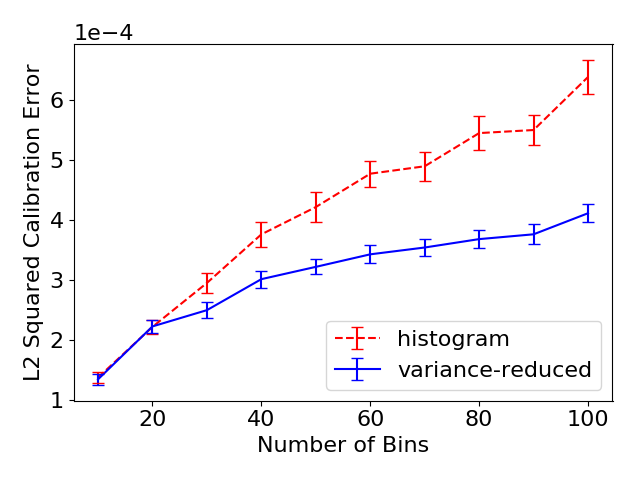
\includegraphics[width=0.8\textwidth]{marginal_ces.png}
         \caption{Effect of number of bins on $\lsquared{}$ calibration error.}
         \label{fig:marginal_calibrator_comparison_cifar}
     \end{subfigure}
     \hfill
     \begin{subfigure}[b]{0.44\textwidth}
         \centering
         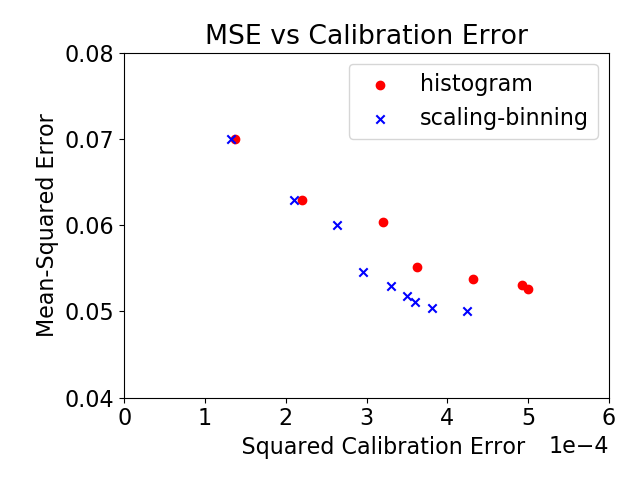
\includegraphics[width=\textwidth]{marginal_mse_vs_ces.png}
         \caption{Tradeoff between calibration and MSE.}
         \label{fig:cifar_calibrator_cmp_mse_ce}
     \end{subfigure}
  \caption{
  (\textbf{Left}) Recalibrating using 1,000 data points on CIFAR-10, our variance-reduced calibrator achieves lower $\lsquared{}$ calibration error than histogram binning, especially when the number of bins $B$ is large.
  (\textbf{Right}) For a fixed calibration error, our variance-reduced calibrator allows us to use more bins. This results in models with more predictive power which can be measured by the mean-squared error. Note the Y-axis range is $[0.4, 0.8]$ to zoom into the relevant region.
  }
  \label{fig:nan2}
\end{figure}
